\documentclass{article}
\usepackage[margin=2cm]{geometry}
\usepackage{graphicx}
\usepackage[pages=some]{background}
\usepackage{titling}
\usepackage{tabularx}
\usepackage{tikz}
\usepackage{forest}

\forestset{
  my box/.style={
    draw,
    rectangle,
    rounded corners,
    fill=gray!20,
    inner sep=6pt,
    minimum width=3cm % Adjust the width as needed
  }
}


\geometry{a4paper}

\backgroundsetup{
    scale=1,
    angle=0,
    opacity=1,
    contents={%
        
\includegraphics[width=\paperwidth,height=\paperheight]{institution_logo.jpg}
    }
}

\newcommand{\subtitle}[1]{
    \posttitle{
        \par\end{center}
        \begin{center}\large#1\end{center}
        \vskip0.5em}
}

\title{ME-415}
\author{Md. Hasibul Islam}
\subtitle{REFRIGERATION \& BUILDING MECHANICAL SYSTEM}

\begin{document}
\begin{titlepage}
    \centering
    
    {\Huge\bfseries\maketitle}
    \textbf{Alok Kumar Majumder Sir} \\
    \vspace{2cm}
    
\includegraphics[width=8cm]{institution_logo.jpg}
    \vfill
    \vspace*{2cm}
\end{titlepage}

\tableofcontents
\pagebreak
\section{Lecture 01: Introduction} 
\hfill Date: 04/06/2023 


\section{Lecture 2: Different Refrigeration System}
\hfill Date: 11/06/2023

\subsection{Vapour Compression Refrigeration System (VCRS)}
The Vapor Compression Refrigeration System is a widely used refrigeration technology that allows for the cooling of spaces, preservation of food, and other applications requiring low temperatures. It operates on the principle of phase change and heat transfer using a refrigerant.Components of a Vapor Compression Refrigeration System:
\begin{itemize}
  \item Compressor: The compressor is the heart of the system. It receives low-pressure refrigerant vapor from the evaporator, and through compression, increases its pressure and temperature. The compressor helps maintain the flow of refrigerant throughout the system.
  \item Condenser: The high-pressure, high-temperature refrigerant vapor leaving the compressor flows into the condenser. In the condenser, the refrigerant releases heat to the surroundings, typically through a heat exchange process with ambient air or water. As a result, the refrigerant condenses into a high-pressure liquid.
  \item Expansion Valve: The high-pressure liquid refrigerant from the condenser enters the expansion valve. The expansion valve reduces the pressure of the refrigerant, causing it to undergo a rapid expansion. This expansion leads to a drop in temperature and pressure as the refrigerant enters the evaporator.
  \item Evaporator: The low-pressure, low-temperature refrigerant from the expansion valve enters the evaporator. In the evaporator, the refrigerant absorbs heat from the surroundings, such as air or the interior of a refrigerator. As the refrigerant absorbs heat, it undergoes a phase change from a low-pressure liquid to a low-pressure vapor.
\end{itemize}

Working of a Vapor Compression Refrigeration System:\\


The system starts with the compressor, which compresses the low-pressure refrigerant vapor, increasing its pressure and temperature. The high-pressure vapor flows into the condenser, where it releases heat to the surroundings and condenses into a high-pressure liquid.


The high-pressure liquid then passes through the expansion valve, where its pressure and temperature decrease. This causes the refrigerant to rapidly expand and cool down. The low-pressure refrigerant enters the evaporator, where it absorbs heat from the surroundings, cooling the space or the items being refrigerated. The refrigerant evaporates in the process, changing back into a low-pressure vapor.


The low-pressure vapor returns to the compressor to repeat the cycle. This continuous circulation of refrigerant allows for the removal of heat from the cooled space and its release to the surroundings.\\ 


Advantages of Vapor Compression Refrigeration System:
\begin{itemize}
  \item Efficient Cooling: The vapor compression cycle is an efficient means of cooling, allowing for effective temperature control.
  \item Versatility: The system can be used for various applications, ranging from household refrigerators to large-scale industrial cooling systems.
  \item Reliability: Vapor compression refrigeration systems are well-established and reliable technologies, widely used in different industries.
  \item Wide Range of Temperatures: The system can achieve a wide range of temperatures, from sub-zero temperatures for freezing applications to moderate cooling for air conditioning.
  \item Availability of Refrigerants: There is a broad range of refrigerants available for use, depending on the specific requirements of the application.
\end{itemize}

\subsection{VCRS Cycle}
\begin{figure}[htbp]
  \centering
  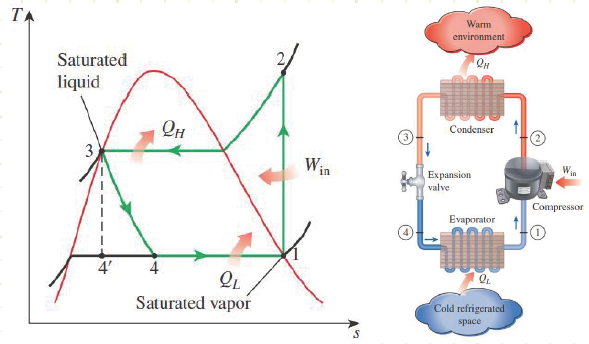
\includegraphics[width=0.85\textwidth]{img/vcrs_cycle.png}
  \caption{Schematic diagram of vapor compression refrigeration cycle}
  \label{fig:vcrs_cycle}
\end{figure}

\subsubsection*{Role of Compressor:}
The compressor plays a crucial role in the vapor compression refrigeration system. Its primary function is to increase the pressure and temperature of the refrigerant vapor, which is essential for the overall operation of the system. Here are the details about the role of the compressor:

\begin{itemize}
  \item Pressure Increase: The compressor receives low-pressure refrigerant vapor from the evaporator. It compresses the vapor, significantly increasing its pressure. This pressure increase is necessary for the refrigerant to release heat effectively in the condenser and enable the subsequent cooling process.
  \item Temperature Increase: As the compressor compresses the refrigerant vapor, it also raises its temperature. The compression process causes the gas molecules in the refrigerant to collide more frequently, resulting in an increase in thermal energy and temperature. This high-temperature refrigerant is then ready to release heat in the condenser.
  \item Maintaining Flow: The compressor maintains the flow of refrigerant throughout the system. By creating a pressure difference, it pushes the refrigerant through the various components, ensuring a continuous circulation of the working fluid. This flow is essential for the proper functioning of the refrigeration cycle.
  \item Overcoming Pressure Drops: In a refrigeration system, there may be pressure drops due to friction or resistance in the piping and components. The compressor compensates for these pressure drops by raising the refrigerant's pressure to ensure efficient operation and maintain the desired temperature differences between components.
  \item Power Consumption: The compressor requires mechanical work to perform its function. It is usually powered by an electric motor or an engine. The power consumed by the compressor is a significant factor in the overall energy consumption of the refrigeration system. Efficient compressor design and operation are important to minimize energy consumption and maximize system performance.
  \item Types of Compressors: There are different types of compressors used in vapor compression refrigeration systems, including reciprocating compressors, rotary compressors, screw compressors, and scroll compressors. Each type has its own advantages and disadvantages, depending on factors such as size, efficiency, cost, and application requirements.
\end{itemize}

\subsubsection*{Role of Condenser:}
The condenser is a vital component of the vapor compression refrigeration system. Its primary role is to facilitate the release of heat absorbed by the refrigerant during the cooling process. Here are the details about the role of the condenser:

\begin{itemize}
  \item Heat Rejection: The condenser receives high-pressure, high-temperature refrigerant vapor from the compressor. Its main function is to transfer heat from the refrigerant to the surroundings. The heat absorbed by the refrigerant during the evaporator stage is released in the condenser, causing the refrigerant to undergo a phase change from a vapor to a liquid.
  \item Heat Transfer: The condenser facilitates heat transfer through various means, such as heat exchange with ambient air or water. Typically, the condenser consists of a network of tubes or coils with fins that increase the heat transfer surface area. As the refrigerant flows through these tubes, it transfers heat to the surrounding medium, resulting in the condensation of the refrigerant vapor.
  \item Cooling Medium: The condenser utilizes a cooling medium, such as air or water, to remove heat from the refrigerant. In air-cooled condensers, ambient air is blown over the condenser coils, causing the refrigerant to release heat and cool down. Water-cooled condensers, on the other hand, circulate water through the condenser tubes, absorbing heat from the refrigerant.
  \item Pressure Reduction: As the refrigerant releases heat in the condenser, it undergoes a pressure reduction. The high-pressure vapor from the compressor transforms into a high-pressure liquid state during condensation. This high-pressure liquid is then sent to the expansion valve for further pressure reduction before entering the evaporator.
  \item Efficiency and Subcooling: The performance of the condenser affects the overall efficiency of the refrigeration system. Efficient heat transfer in the condenser is crucial to achieve effective cooling and ensure optimal energy usage. Additionally, some condensers are designed to provide subcooling, where the temperature of the condensed refrigerant is further reduced below its saturation temperature. Subcooling enhances the system's performance by preventing any flash vaporization before the refrigerant enters the expansion valve.
  \item Types of Condensers: Various types of condensers are used in vapor compression refrigeration systems, including air-cooled condensers, water-cooled condensers, and evaporative condensers. Each type has its own advantages and suitability for specific applications, considering factors such as space availability, cooling medium availability, and environmental conditions.
\end{itemize}


\subsubsection*{Role of Expansion Valve:}
The expansion valve, also known as the throttle valve or metering device, is a crucial component in the vapor compression refrigeration system. Its primary role is to regulate the flow of high-pressure liquid refrigerant from the condenser to the evaporator. Here are the details about the role of the expansion valve:

\begin{itemize}
  \item Pressure Reduction: The expansion valve reduces the pressure of the high-pressure liquid refrigerant coming from the condenser. This pressure reduction is essential for the refrigerant to undergo a phase change from a liquid to a vapor in the evaporator. By reducing the pressure, the expansion valve enables the refrigerant to expand and evaporate at a lower temperature.
  \item Temperature Drop: As the expansion valve reduces the pressure of the refrigerant, it also causes a significant drop in temperature. This drop in temperature occurs due to the relationship between pressure and temperature in the refrigeration cycle. The expansion valve creates an abrupt pressure drop, leading to a corresponding temperature decrease, which prepares the refrigerant for the evaporator's cooling process.
  \item Flow Control: The expansion valve acts as a flow control device, regulating the rate at which the high-pressure liquid refrigerant enters the evaporator. By adjusting the size of the valve opening, the flow of refrigerant can be precisely controlled, matching the cooling load requirements of the system. This flow control ensures optimal performance and efficiency.
  \item Ensuring Proper Evaporation: The expansion valve ensures that the refrigerant enters the evaporator as a mixture of liquid and vapor. This controlled mixture facilitates efficient heat transfer between the refrigerant and the surroundings (e.g., air or the interior of a refrigerated space). The liquid portion of the refrigerant absorbs heat, evaporating and cooling the surroundings, while the vapor portion continues to evaporate as it absorbs more heat.
  \item Superheat Control: The expansion valve helps maintain the desired level of superheat in the evaporator. Superheat refers to the temperature of the refrigerant vapor above its boiling point. By carefully controlling the flow of refrigerant, the expansion valve can adjust the amount of superheat in the evaporator, ensuring efficient heat transfer and preventing issues such as liquid refrigerant carryover to the compressor.
  \item Types of Expansion Valves: Different types of expansion valves are used in vapor compression refrigeration systems, including thermostatic expansion valves (TXV), electronic expansion valves (EEV), and capillary tubes. Each type has its own design and mode of operation, offering specific advantages and suitability for different applications.
\end{itemize}

\subsubsection*{Role of Evaporator:}
The evaporator is a crucial component in the vapor compression refrigeration system. Its primary role is to absorb heat from the surroundings, such as air or the interior of a refrigerated space, and facilitate the evaporation of the low-pressure liquid refrigerant. Here are the details about the role of the evaporator:

\begin{itemize}
  \item Heat Absorption: The evaporator is responsible for absorbing heat from the surroundings that need to be cooled. This can be the air in an air conditioning system or the interior of a refrigerator. As the low-pressure liquid refrigerant enters the evaporator, it flows through a network of tubes or coils designed to maximize the contact surface area with the surroundings. The absorbed heat causes the refrigerant to evaporate, changing its state from a liquid to a vapor.
  \item Cooling Effect: As the low-pressure liquid refrigerant evaporates, it extracts heat from the surrounding environment, resulting in a cooling effect. The heat absorbed causes the refrigerant to undergo a phase change, absorbing thermal energy from the surroundings and reducing their temperature. This cooling effect is what provides the desired refrigeration or air conditioning in the system.
  \item Boiling Process: The evaporator facilitates the boiling process of the refrigerant. The low-pressure liquid refrigerant boils, or evaporates, as it absorbs heat from the surroundings. The refrigerant takes in the energy required for the phase change, transforming into a low-pressure vapor while cooling the surrounding environment.
  \item Superheat Control: The evaporator plays a role in controlling the level of superheat in the refrigerant vapor. Superheat refers to the temperature of the refrigerant vapor above its boiling point. It is important to maintain a certain level of superheat to prevent any liquid refrigerant from entering the compressor, as it could damage the compressor. Proper design and control of the evaporator ensure that the refrigerant leaving the evaporator is in a vapor state with the desired level of superheat.
  \item Heat Transfer Surface: The evaporator is designed with a large heat transfer surface area to maximize the heat exchange between the refrigerant and the surroundings. This is typically achieved through the use of finned tubes or coils that increase the surface area and promote efficient heat transfer.
  \item Return of Refrigerant: Once the refrigerant has absorbed heat and evaporated in the evaporator, it exits the evaporator as a low-pressure vapor and returns to the compressor to repeat the refrigeration cycle. The vapor is then compressed, leading to an increase in pressure and temperature before it enters the condenser.
\end{itemize}

\section{Vapor Absorption Refrigeration System}

The vapor absorption refrigeration system is an alternative to the more common vapor compression refrigeration system. It operates on a different principle, using a combination of an absorbent and a refrigerant to achieve cooling. Generally, water is used as an absorbant, and $NH_3$ is used as a refrigerant or coolant.\\

\begin{figure}[htbp]
  \centering
  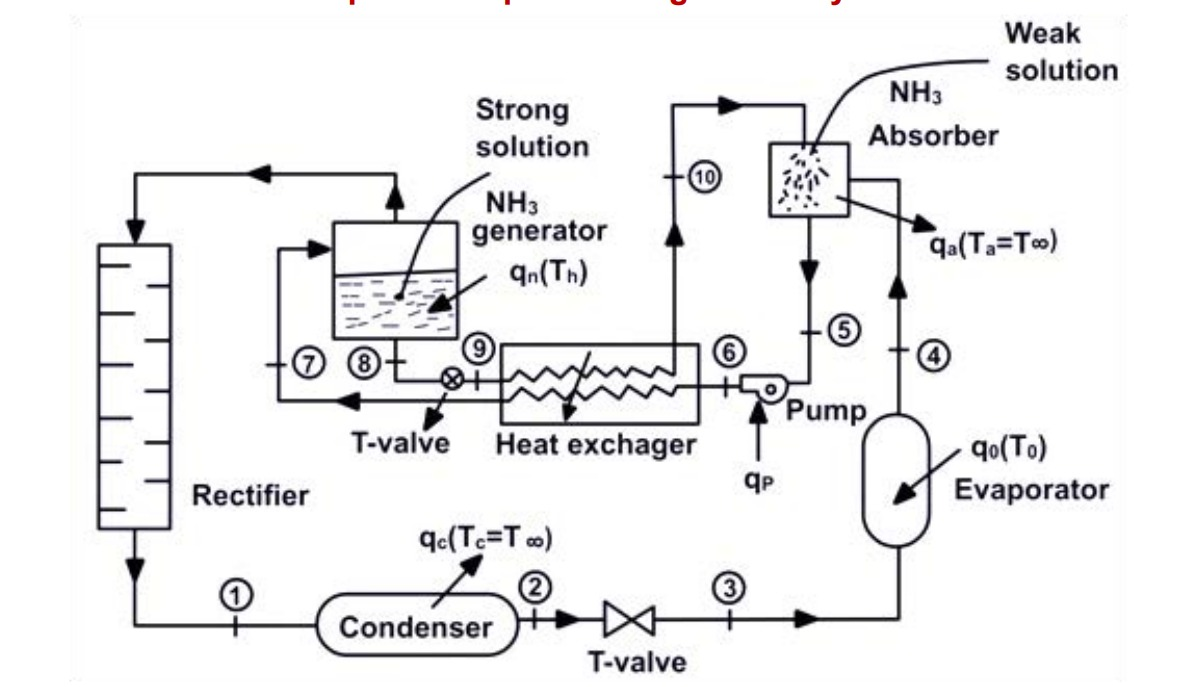
\includegraphics[width=0.85\textwidth]{img/vars_cycle.png}
  \caption{Schematic diagram of vapor absorption refrigeration cycle}
  \label{fig:vars_cycle}
\end{figure}

Components of a Vapor Absorption Refrigeration System:\\

\begin{itemize}
  \item Absorber: The absorber is where the refrigerant vapor is absorbed into a liquid absorbent. The absorbent typically has a high affinity for the refrigerant vapor, allowing it to dissolve and form a concentrated solution.
  \item Generator: The generator is responsible for separating the refrigerant from the absorbent solution. This is achieved by heating the solution, causing the refrigerant to vaporize while the absorbent remains in liquid form. The vaporized refrigerant is then directed to the condenser.
  \item Condenser: The vaporized refrigerant from the generator enters the condenser, where it releases heat to the surroundings. This heat transfer causes the refrigerant vapor to condense into a high-pressure liquid.
  \item Expansion Valve: The high-pressure liquid refrigerant from the condenser passes through the expansion valve, which reduces its pressure and temperature. This pressure reduction allows the refrigerant to expand and cool down, preparing it for the evaporator.
  \item Evaporator: The low-pressure, low-temperature refrigerant from the expansion valve enters the evaporator. In the evaporator, the refrigerant absorbs heat from the surroundings, such as air or a refrigerated space. The absorbed heat causes the refrigerant to evaporate, changing it back into a low-pressure vapor.
\end{itemize}


Advantages of Vapor Absorption Refrigeration System:\\

\begin{itemize}
  \item Environmentally Friendly: The vapor absorption refrigeration system typically uses natural refrigerants and non-toxic absorbents, making it more environmentally friendly than systems that use synthetic refrigerants.
  \item Utilization of Low-Grade Heat: The system can utilize waste heat or low-grade heat sources for the desorption process in the generator. This makes it suitable for applications where such heat sources are available, leading to energy savings.
  \item Quiet Operation: The vapor absorption refrigeration system operates without a mechanical compressor, resulting in quieter operation compared to vapor compression systems.
  \item Flexibility in Energy Sources: The system can operate using various energy sources for heating, such as natural gas, waste heat, solar energy, or geothermal energy, offering flexibility in energy options.
\end{itemize}


Disadvantages of Vapor Absorption Refrigeration System:\\
\begin{itemize}
  \item Lower Efficiency: The vapor absorption refrigeration system generally has lower efficiency compared to vapor compression systems. This is due to the additional energy required for the desorption process and the use of higher temperatures in the generator.
  \item Larger Footprint: The system typically requires larger equipment and a larger physical footprint compared to vapor compression systems, making it less suitable for space-constrained applications.
  \item Higher Initial Cost: The initial cost of the vapor absorption refrigeration system is often higher due to the complex design and specialized components required.
\end{itemize}


Applications of Vapor Absorption Refrigeration System:\\
The vapor absorption refrigeration system is commonly used in various applications, including:\\
\begin{itemize}
  \item Industrial Cooling: It is used for industrial cooling processes that require larger cooling capacities, such as food processing, chemical plants, and refrigeration in large-scale facilities.
  \item Air Conditioning: The system is suitable for air conditioning in commercial buildings, hotels, and other spaces where waste heat or low-grade heat sources are available.
  \item Refrigeration in Remote Locations: The system is utilized in remote locations or off-grid areas where electricity supply is limited or unreliable. It can operate using alternative energy sources such as natural gas or solar energy.
  \item Cooling in Absence of Electricity: The vapor absorption refrigeration system is useful in locations where electricity is not available or during power outages. It can operate using heat sources like biomass or gas burners.
\end{itemize}



\subsubsection*{Overall Processes of VARS:}
\begin{itemize}
  \item Generator: An external heating source is used to heat the strong solution of ammonia (NH3), producing ammonia vapor at high pressure. The ammonia vapor carries water vapor, which is subsequently removed in the rectifier.
  \item Rectifier: This component separates the water vapor from the ammonia vapor, ensuring that only dehydrated ammonia gas enters the condenser.
  \item Condenser: High-pressure ammonia vapor is condensed in the condenser, releasing heat and converting it into a high-pressure liquid ammonia.
  \item Throttle Valve: The cooled ammonia solution passes through a throttle valve, which reduces the pressure and temperature of the refrigerant below the desired temperature in the evaporator. This creates a low-temperature refrigerant.
  \item Evaporator: The low-temperature refrigerant enters the evaporator, where it absorbs heat from the surroundings, typically a space to be cooled. The refrigerant evaporates, leaving the evaporator as saturated vapor.
  \item Absorber: Slightly superheated, low-pressure ammonia vapor from the evaporator is absorbed by a weak solution of ammonia (aqua-ammonia) in the absorber. The weak solution, after absorbing ammonia vapor, becomes a strong solution.
  \item Pump: The strong ammonia solution, now at high pressure, is pumped back to the generator through a heat exchanger. The pump increases the pressure of the strong solution to the generator pressure.
  \item Heat Exchanger: The heat exchanger facilitates heat transfer between the high-temperature weak ammonia solution coming from the generator and the strong ammonia solution from the absorber. This process helps maintain the temperature difference required for efficient absorption in the absorber.
  \item Throttle Valve (again): The weak high-temperature ammonia solution from the generator is passed through the throttle valve, reducing its pressure to match the absorber pressure.
\end{itemize}

This completes the cycle of the vapor absorption refrigeration system, where heat is absorbed in the evaporator and released in the generator, utilizing the absorption-desorption process of ammonia and the transfer of heat through various components.

\pagebreak


\subsection*{Difference between VCRS and VARS:}

\begin{table}[!htbp]
  \centering
  \begin{tabularx}{\linewidth}{@{}>{\hsize=0.6\hsize}X *{2}{>{\hsize=1.2\hsize}X}@{}}
    \hline
    \textbf{Differences} & \textbf{Vapor Compression Refrigeration system} & \textbf{Vapor Absorption Refrigeration system} \\
    \hline
    Working Principle & The vapor compression refrigeration system operates based on the compression and expansion of a refrigerant vapor. It uses a mechanical compressor to increase the pressure and temperature of the refrigerant vapor, followed by condensation, expansion, and evaporation stages. & The vapor absorption refrigeration system utilizes a combination of an absorbent and a refrigerant to achieve cooling. It relies on the absorption and desorption of the refrigerant by an absorbent, followed by condensation, expansion, and evaporation stages. \\
    \hline 
    Energy Input & The vapor compression system requires a significant amount of mechanical energy to operate the compressor, which increases the pressure and temperature of the refrigerant vapor. & The vapor absorption system relies on heat input for the desorption process, where the refrigerant vapor is separated from the absorbent. This heat input can come from waste heat, low-grade heat sources, or other forms of thermal energy.\\
    \hline 
    Energy Efficiency & The vapor compression system generally has higher energy efficiency compared to the vapor absorption system. It benefits from advancements in compressor technology and optimized system designs. & The vapor absorption system typically has lower energy efficiency due to the additional energy required for the desorption process and the use of higher temperatures in the generator. However, it can utilize waste heat or low-grade heat sources, leading to overall energy savings. \\
    \hline 
    Environmental Impact & The vapor compression system commonly uses synthetic refrigerants, such as hydrofluorocarbons (HFCs), which have a high global warming potential. The leakage of these refrigerants can contribute to environmental damage. & The vapor absorption system can utilize natural refrigerants, such as ammonia (NH3) or water (H2O), which have low or zero global warming potential. This makes the vapor absorption system more environmentally friendly.\\
    \hline 
    Applications & The vapor compression system is widely used in various applications, including residential and commercial air conditioning, refrigeration in supermarkets, food processing, and industrial cooling. & The vapor absorption system is commonly employed in specific applications, such as large-scale industrial cooling processes, air conditioning in commercial buildings with waste heat available, or cooling in remote locations without reliable electricity supply. \\
    \hline 
    Complexity and Cost & The vapor compression system is generally more compact and less complex, resulting in lower initial equipment costs. It benefits from the widespread use of standardized components and established manufacturing processes. & The vapor absorption system is typically larger and more complex, requiring specialized components and design considerations. This often leads to higher initial costs. \\ 
    \hline
  \end{tabularx}
  \caption{Difference between Vapor Compression Refrigeration System and Vapor Absorption Refrigeration System }
  \label{tab:full-width-table}
\end{table}

\pagebreak
\section{Lecture 04: Types of Refrigeration} 
\hfill Date: 26/06/2023 

\textbf{Online class!! See SLIDE!!}
\vspace*{2cm}

\section{Lecture 05: Magnetic, Vortex tube \& Air cycle Refrigeration} 
\hfill Date: 09/07/2023 

\begin{itemize}
  \item Magnetic Refrigeration 
  \item Vortex Tube Refrigeration
  \item Air Cycle Refrigeration 
\end{itemize}

\textbf{Follow slide or BOOK for understanding!!!} \\

\subsection*{Important Points}
\begin{itemize}
  \item Sea divers uses vortex tube refrigeration inside low temperature ocean. There are hot and cold two region in refrigerator. By hot region, a comfortable temperature is maintained to the divers. 
  \item The boiling temperature of air is -178 °C. So, in room temperature air is in superheated condition. That's why we can not see air by eyes, also can not perceive vortex. 
\end{itemize}

\end{document}
